\documentclass[english,11pt,a4paper]{article}
\usepackage[T1]{fontenc}
\usepackage{graphicx}
\usepackage{mathtools}
\usepackage{amssymb}
\usepackage{amsthm}
\usepackage{thmtools}
\usepackage{xcolor}
\usepackage{nameref}
\usepackage{babel}
\usepackage{authblk}
\usepackage{fourier}
\usepackage{indentfirst}
\usepackage{float}
\usepackage{subcaption}
\usepackage[colorlinks, urlcolor=blue]{hyperref}
\title{Introdução à Neurociência Computacional\\Lista de Exercícios 4}
\author{Paulo R. Sturion}
\begin{document}
	\maketitle
	
	\noindent Todos os códigos escritos para produzir os resultados dos exercícios a seguir estão disponibilizados de forma clara e organizada no repositório Github:
	
	\begin{center}
		\noindent \href{https://github.com/prsturion/intro-computational-neurosciene.git}{https://github.com/prsturion/intro-computational-neuroscience.git} \newline
	\end{center}
	
	\noindent \textbf{Questão 1.} Para valores de \(V\) entre -85 e 50 mV e de \([Ca]\) entre 0 e \(2 \times 10^{-3}\) M, gere gráficos para as 12 constantes de taxa das variáveis de \textit{gating} do modelo de Pinsky-Rinzel.
	
	\begin{figure}[H]
		\centering
		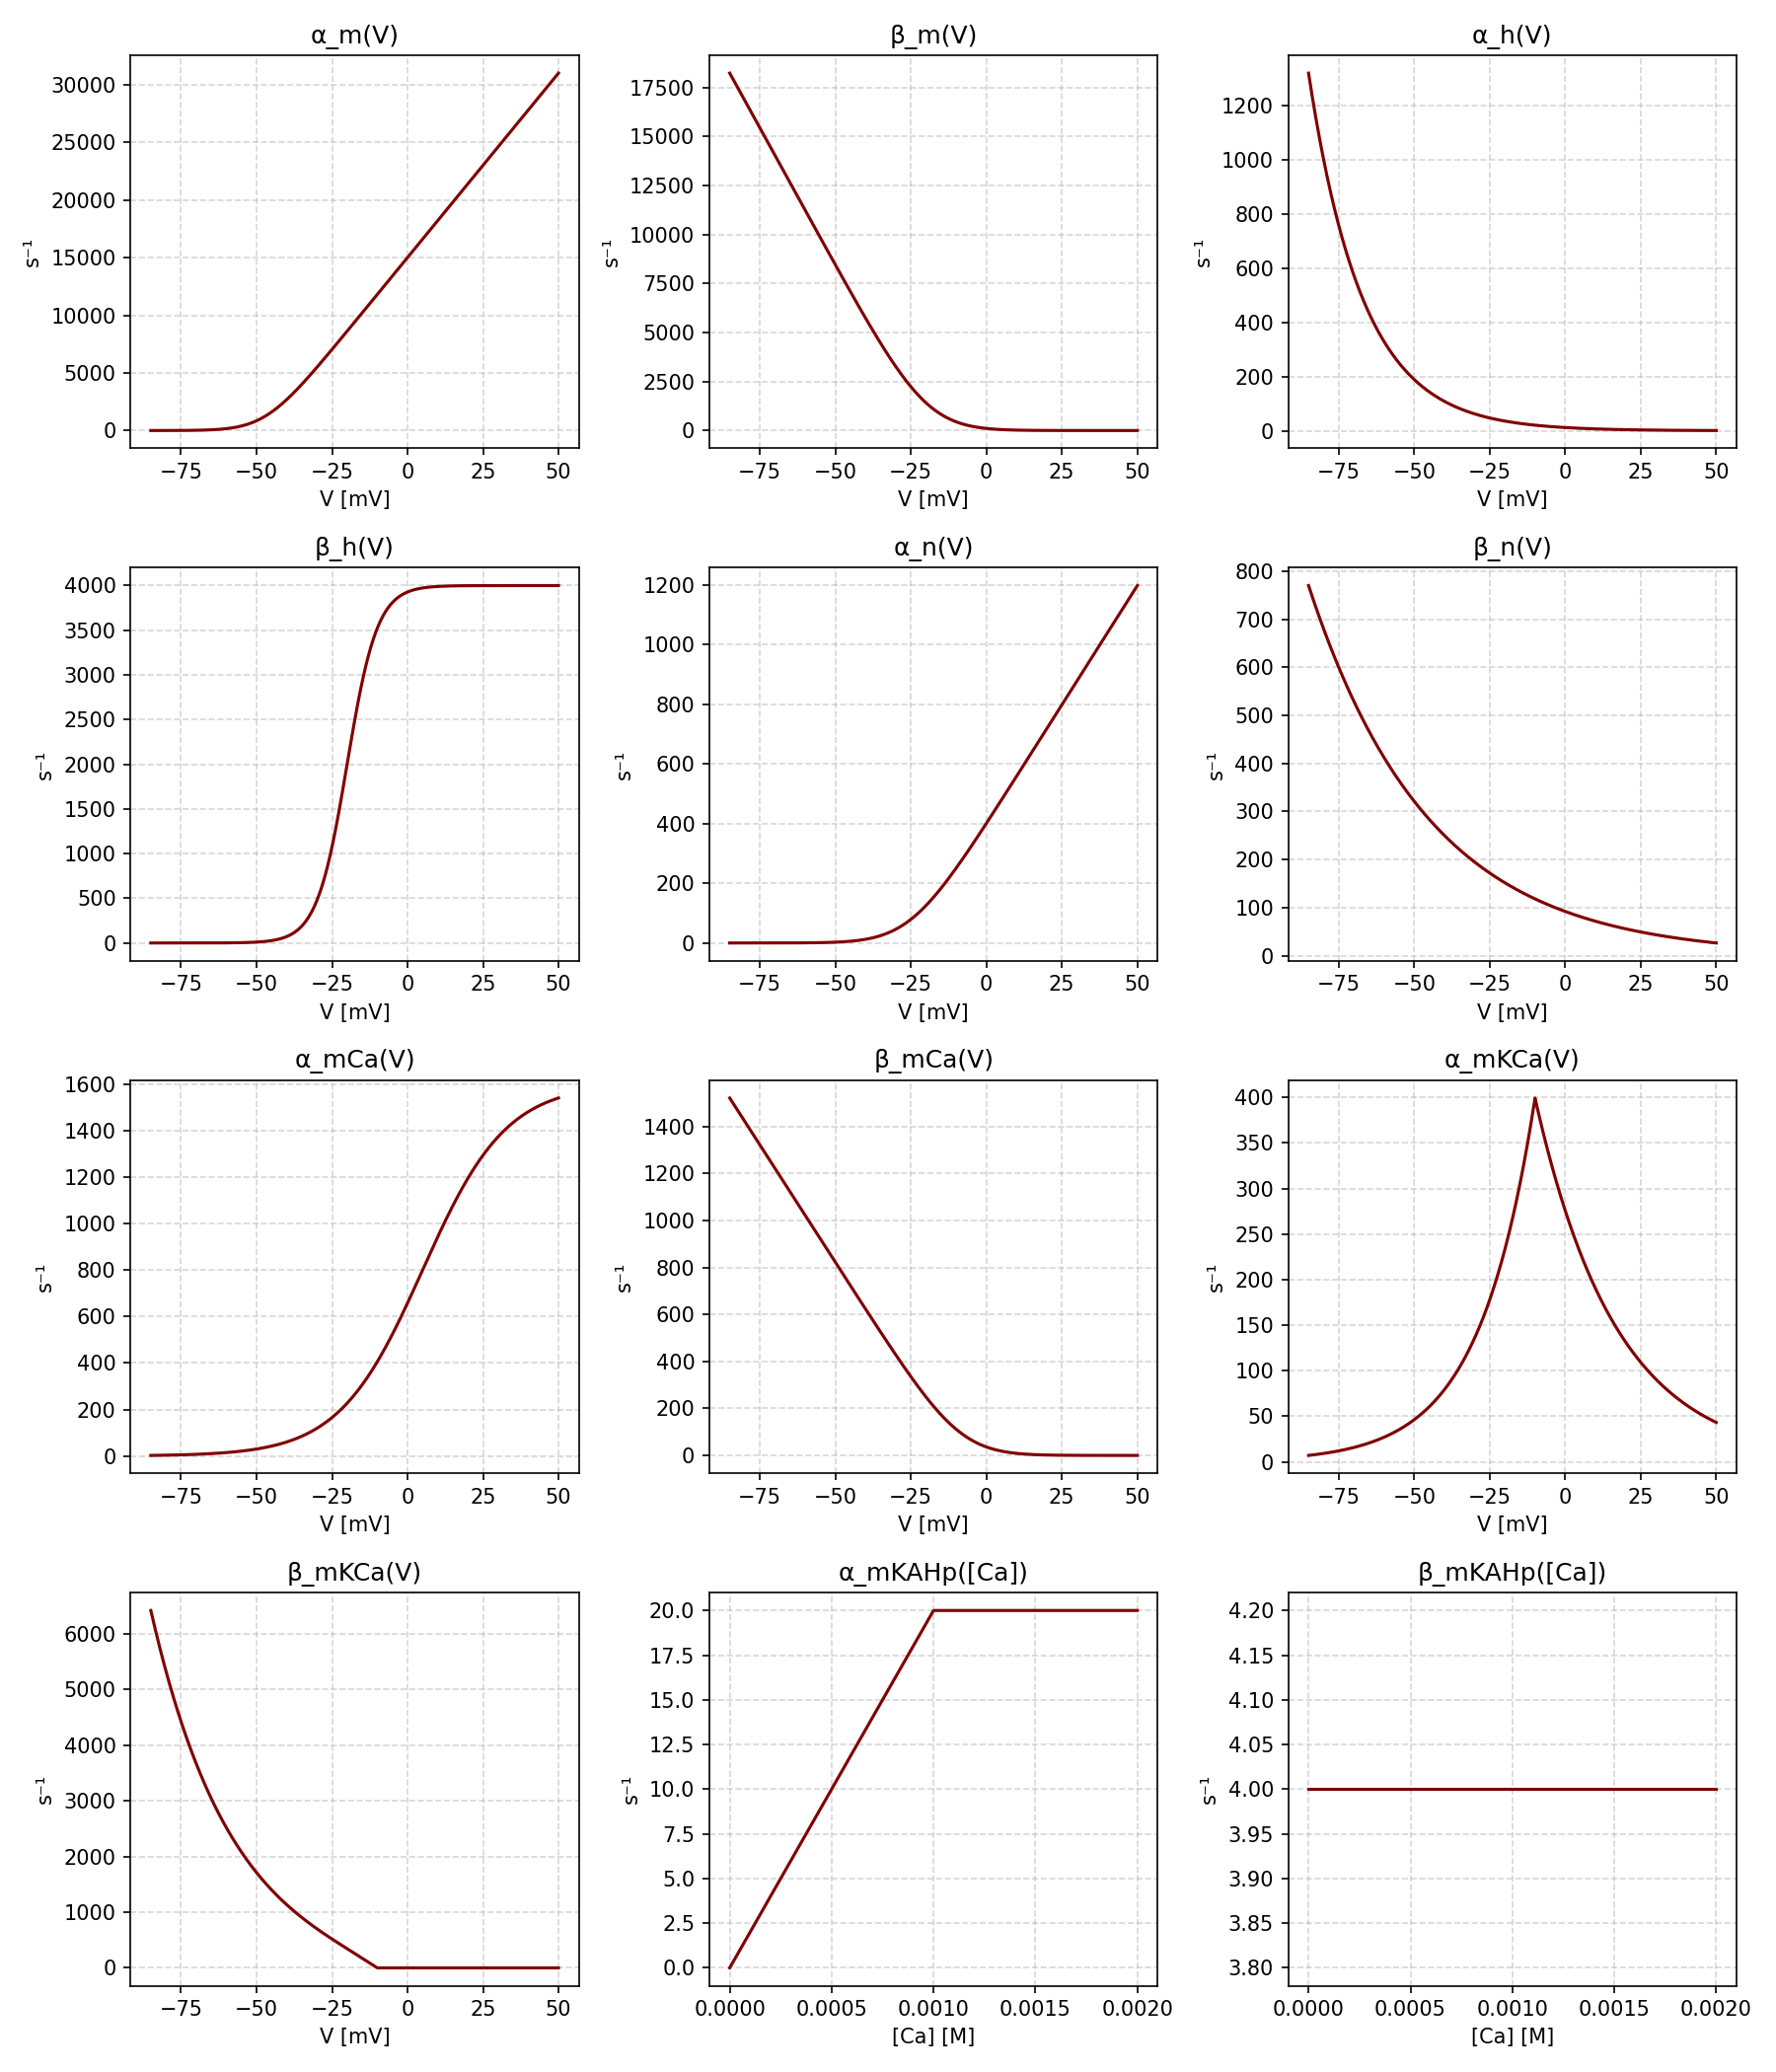
\includegraphics[width=12cm]{../figures/ex_1.png}
		\caption{Gráficos para as 12 constantes de taxa das variáveis de \textit{gating} do modelo Pinsky-Rinzel.}
	\end{figure}
	
	\noindent \textbf{Questão 2.} Simule o modelo com as equações e parâmetros dados acima para \(t\) entre 0 e 2 s. Gere como resultados de sua simulação gráficos que se pareçam com os das Figuras 2 e 3. As Figuras 2 e 3 são cópias escaneadas das Figuras 4.15 e 4.16 do livro de Miller mencionando acima (as figuras foram escaneadas com um celular, por isso estão tortas). Interprete os resultados. Para detectar um disparo somático, use o mesmo critério adotado por Miller: um disparo ocorre quando \(V_s\) ultrapassa -10 mV e um novo disparo só pode acontecer depois que o potencial de membrana retorna para um valor abaixo de -30 mV.
	
	\begin{figure}[H]
		\centering
		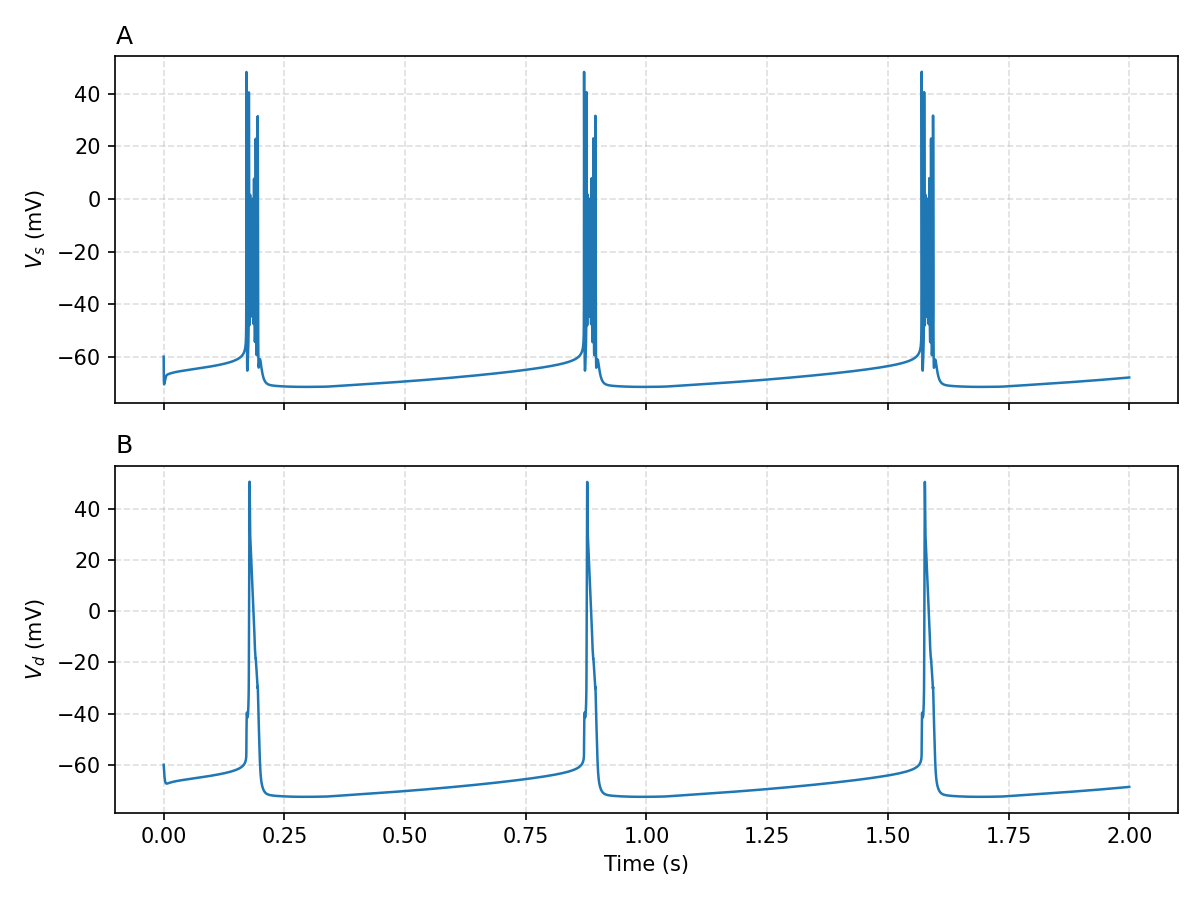
\includegraphics[width=12cm]{../figures/ex_2_1.png}
		\caption{Gráficos de disparos no soma e no dendrito do modelo Pinsky-Rinzel para os parâmetros dados.}
	\end{figure}
	
	
	
	\begin{figure}[H]
		\centering
		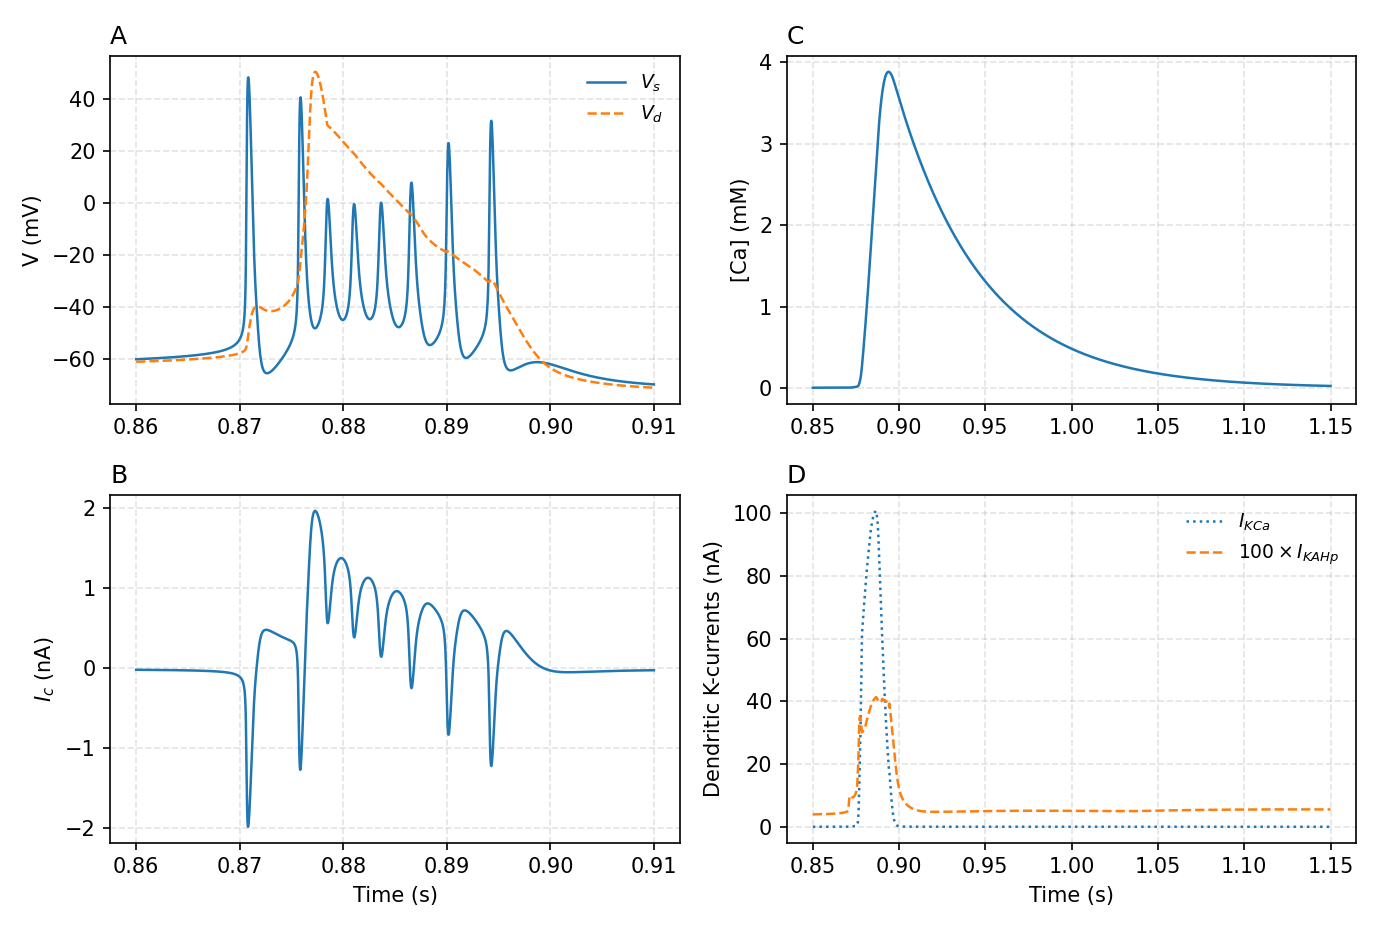
\includegraphics[width=12cm]{../figures/ex_2_2.png}
		\caption{Detalhes do modelo Pinsky-Rinzel durante uma rajada de disparos.}
	\end{figure}
	
	Como pode ser visto tanto na figura do enunciado, quanto no gráfico obtido na simulação, os disparos no dendrito são únicos, enquanto no soma são em rajadas. Isso é coerente com o fato dos canais de cálcio presentes no dendrito serem de cinética lenta, enquanto os canais predominantes de sódio e potássio do soma são de cinética rápida, e conseguem dar vários disparos no tempo de um único disparo dendrítico.\\\\
	

	
	\noindent \textbf{Questão 3.} Faça um estudo de como o comportamento do modelo depende do valor da condutância de acoplamento \(G_c\). Para isso, simule o seu modelo para quatro valores diferentes de \(G_c\) (além do que você já usou na questão 2): 0, 10 nS, 50 nS e 100 nS. Explique as diferenças de comportamento observadas usando gráficos apropriados para sustentar seus argumentos.
	
	\begin{figure}[H]
		\centering
		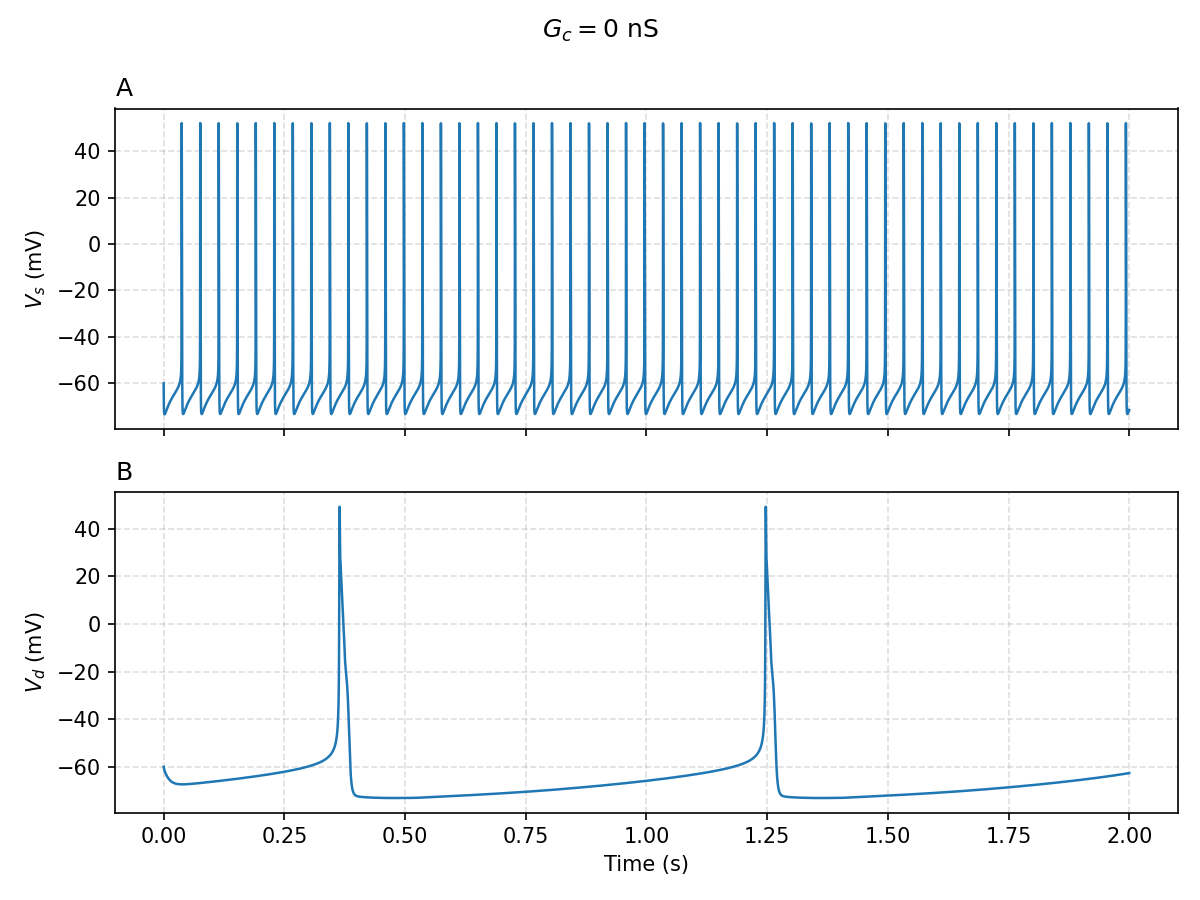
\includegraphics[width=12cm]{../figures/ex_3_gc0.png}
		\caption{Gráficos de disparos no soma e no dendrito para $G_c = 0$ nS.}
	\end{figure}
	
	\begin{figure}[H]
		\centering
		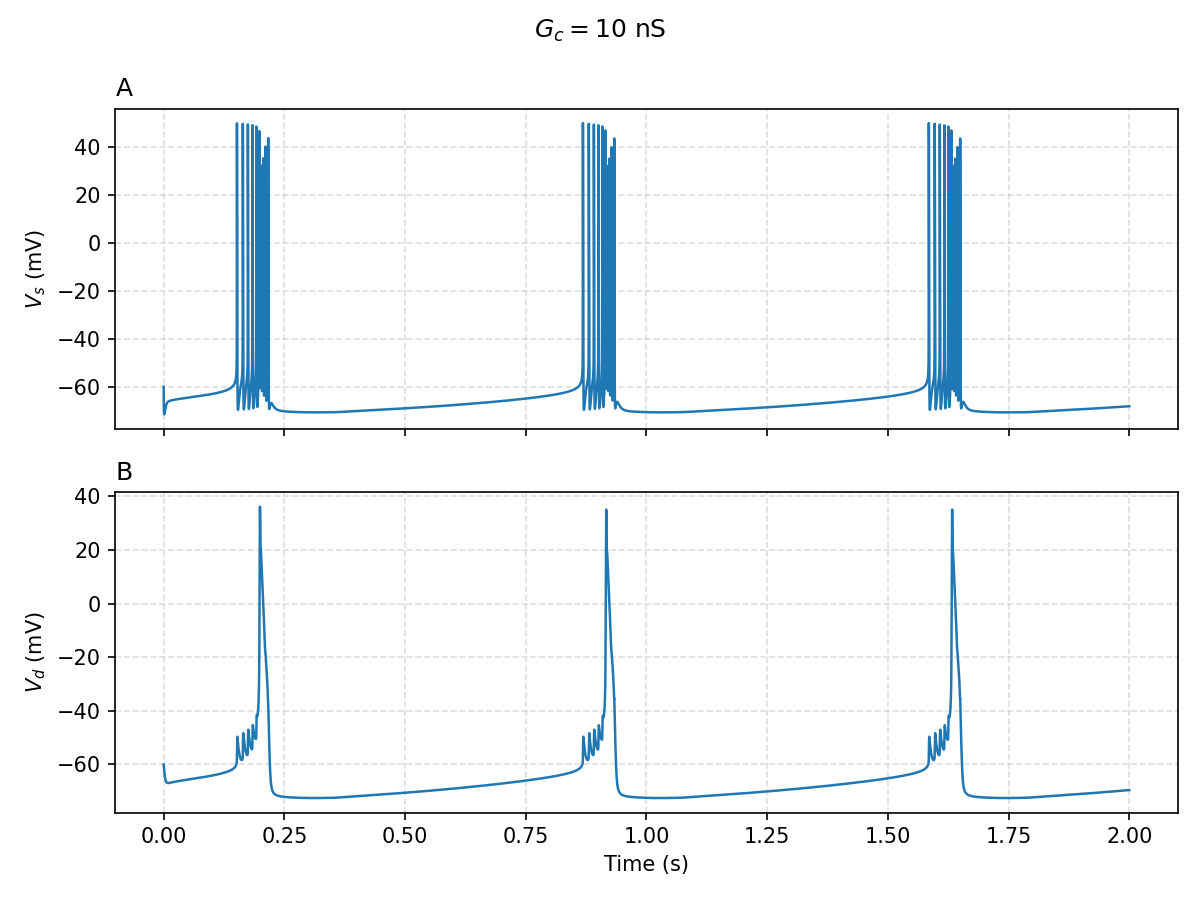
\includegraphics[width=12cm]{../figures/ex_3_gc10.png}
		\caption{Gráficos de disparos no soma e no dendrito para $G_c = 10$ nS.}
	\end{figure}
	
	\begin{figure}[H]
		\centering
		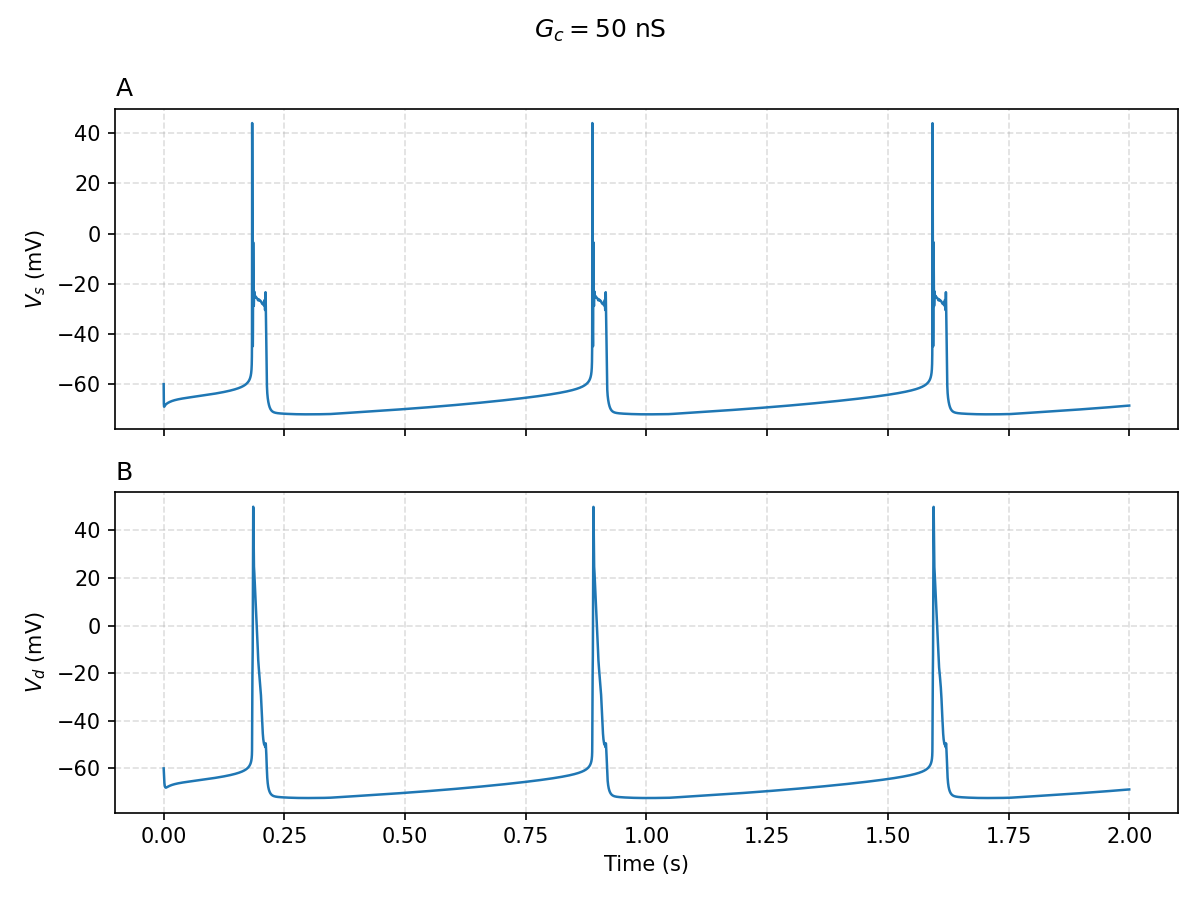
\includegraphics[width=12cm]{../figures/ex_3_gc50.png}
		\caption{Gráficos de disparos no soma e no dendrito para $G_c = 50$ nS.}
	\end{figure}
	
	\begin{figure}[H]
		\centering
		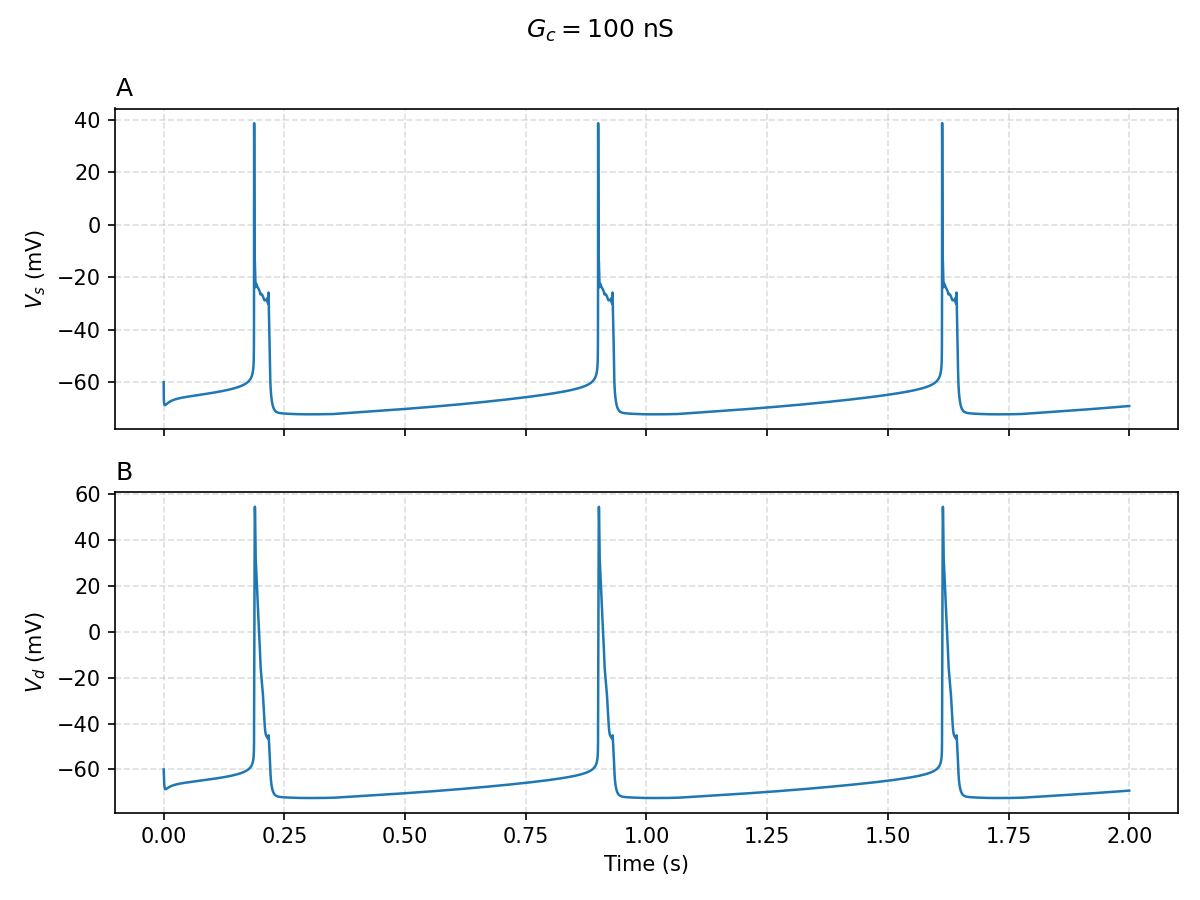
\includegraphics[width=12cm]{../figures/ex_3_gc100.png}
		\caption{Gráficos de disparos no soma e no dendrito para $G_c = 100$ nS.}
	\end{figure}
	
	A diferença entre os gráficos pode ser explicada da seguinte forma. No primeiro, os compartimentos estão desacoplados ($G_c = 0$ nS), logo, cada um segue sua dinâmica natural, com o dendrito tendo seus disparos de cinética lenta, e o soma de cinética rápida. Para valores de $G_c$ baixos, como no segundo gráfico, já é possível ver como um compartimento influencia no outro, sendo que disparos em um, causam a entrada de corrente $I_c$ no outro, e consequentes despolarizações e mudanças na dinâmica. Veja como os disparos do soma agora são mais concentrados juntos aos disparos do dendrito (devida a despolarização intensa concentrada naquele instante, seguida de um período refratário), e veja como os disparos do dendrito possui agora pequenas oscilações na subida causadas pelos disparos rápidos do soma. Por último, para $G_c$ alto, os compartimentos passam a diferir pouco devido a grande comunicação entre eles; como se fossem um único compartimento.\\\\
	
	
	
	\noindent \textbf{Questão 4.} Repita o que foi feito na questão 3 com o fator de conversão \(k\) dobrado: \(k = 5 \times 10^6 / (1 - p)\) M/C. Comente caso haja qualquer mudança observada em relação ao comportamento do modelo na questão 3.
	
	\begin{figure}[H]
		\centering
		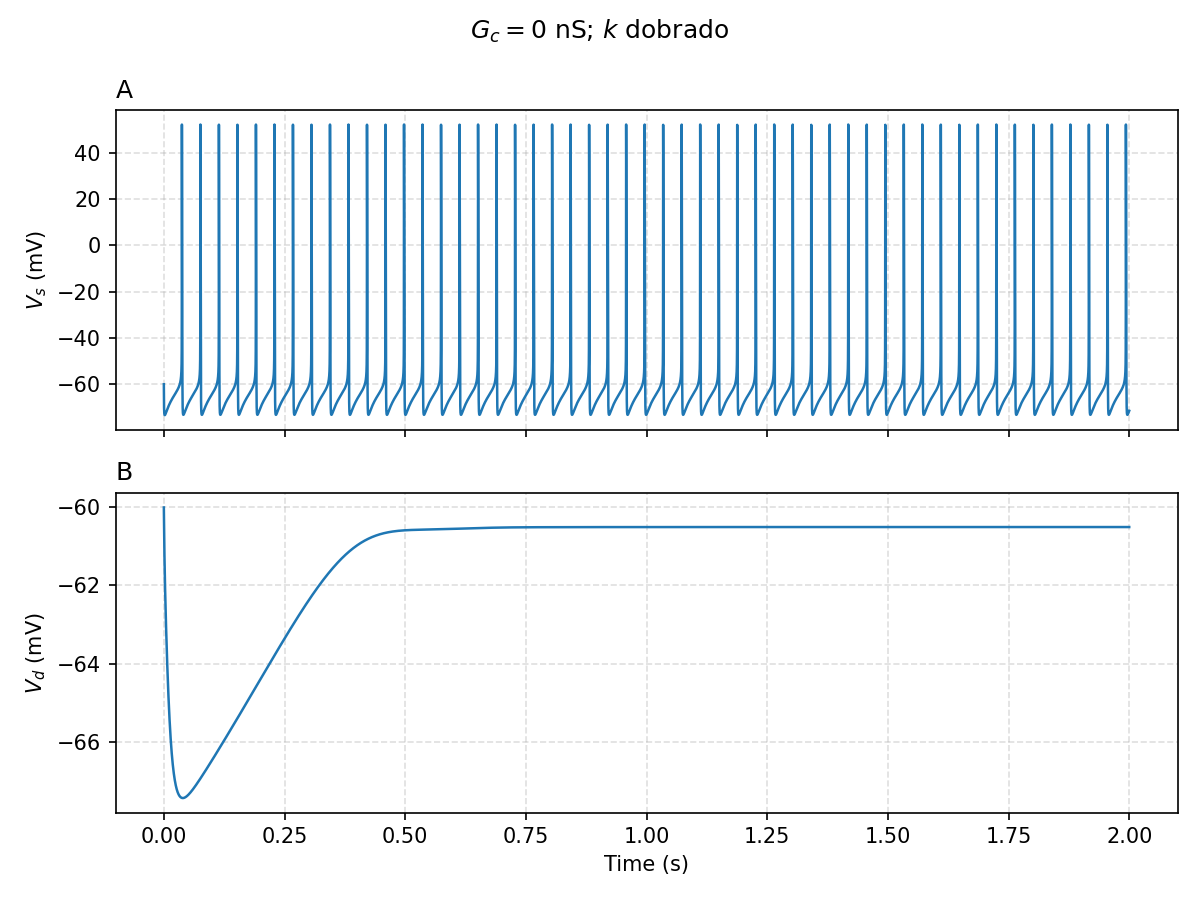
\includegraphics[width=12cm]{../figures/ex_4_gc0.png}
		\caption{Gráficos de disparos no soma e no dendrito para $G_c = 0$ nS com $k$ dobrado.}
	\end{figure}
	
	\begin{figure}[H]
		\centering
		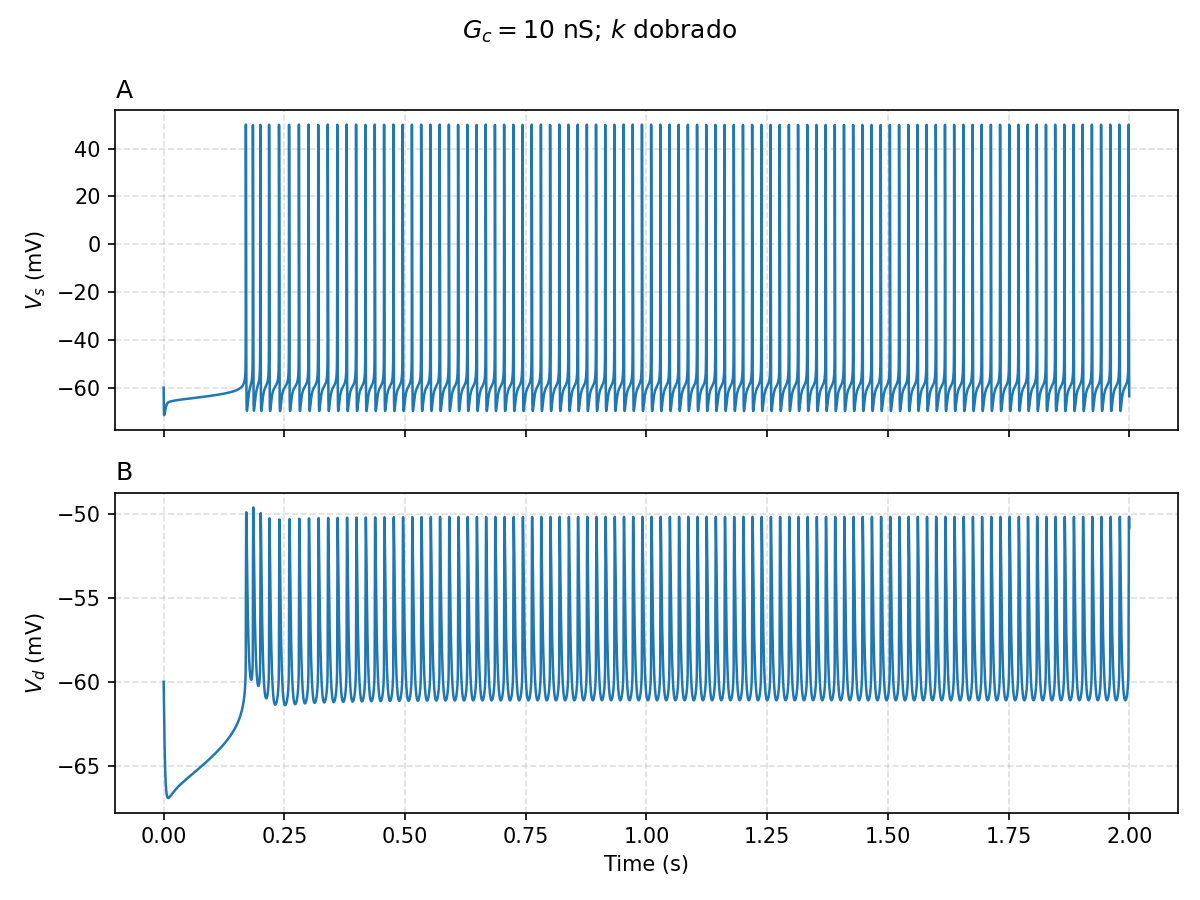
\includegraphics[width=12cm]{../figures/ex_4_gc10.png}
		\caption{Gráficos de disparos no soma e no dendrito para $G_c = 10$ nS com $k$ dobrado.}
	\end{figure}
	
	\begin{figure}[H]
		\centering
		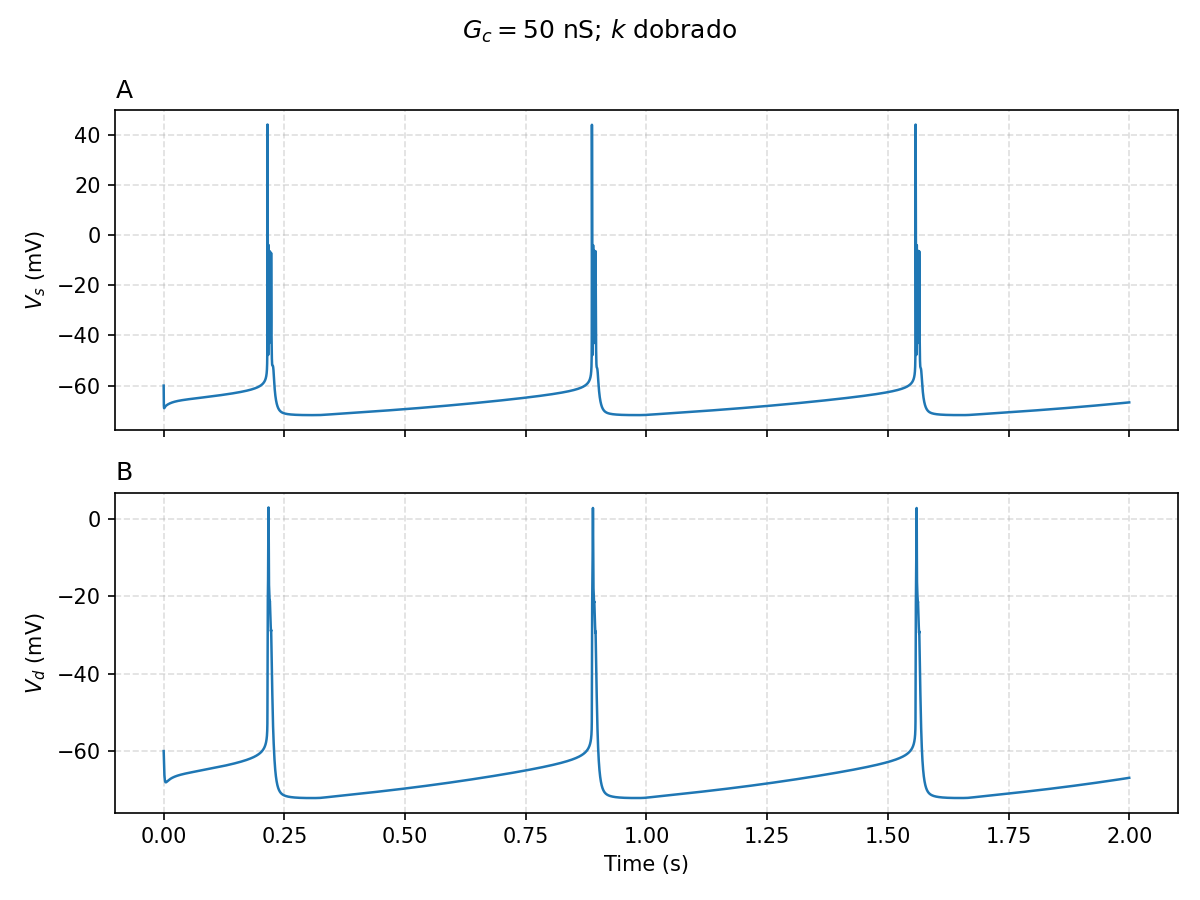
\includegraphics[width=12cm]{../figures/ex_4_gc50.png}
		\caption{Gráficos de disparos no soma e no dendrito para $G_c = 50$ nS com $k$ dobrado.}
	\end{figure}
	
	\begin{figure}[H]
		\centering
		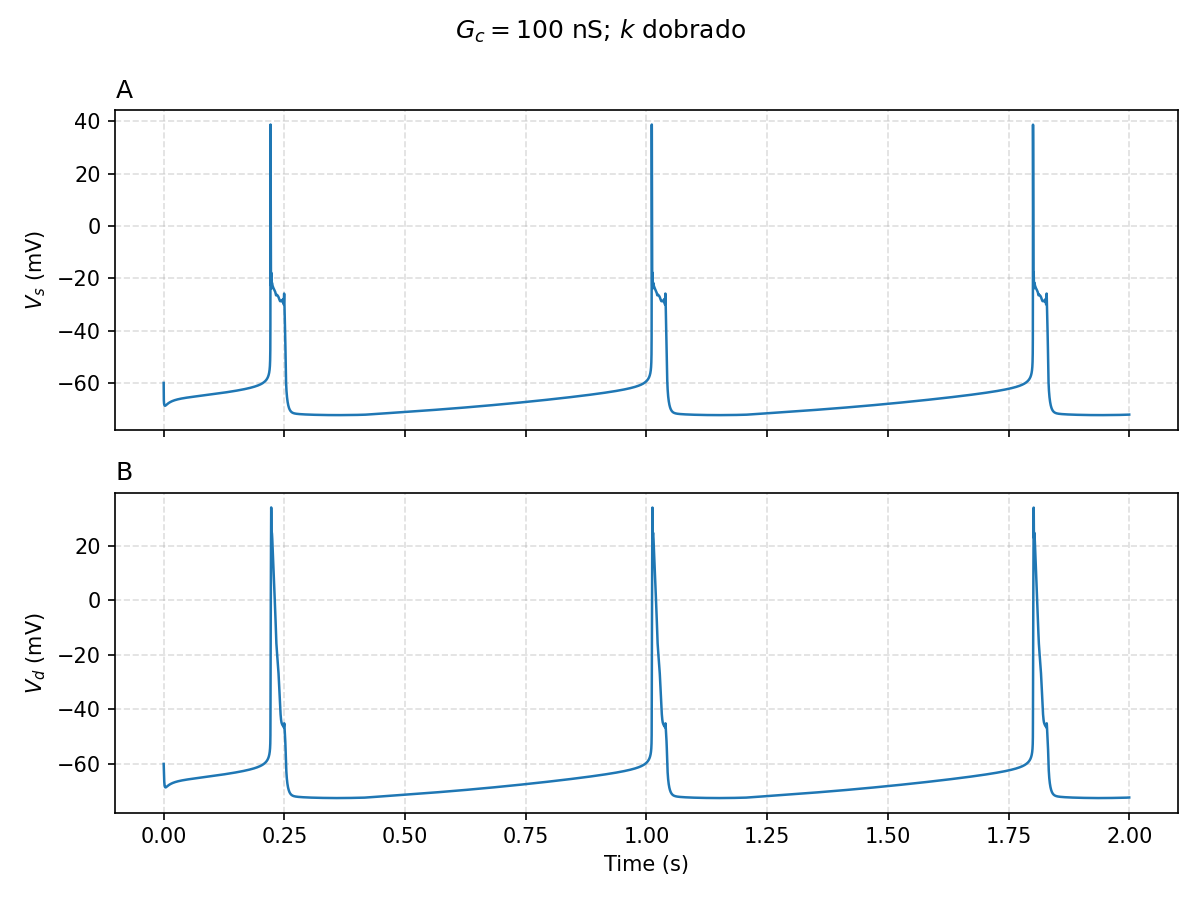
\includegraphics[width=12cm]{../figures/ex_4_gc100.png}
		\caption{Gráficos de disparos no soma e no dendrito para $G_c = 100$ nS com $k$ dobrado.}
	\end{figure}
	
	Essencialmente, ao dobrar o fator $k$, a mesma corrente de cálcio gera um aumento mais rápido na concentração intracelular [Ca]. Isso acelera a ativação dos canais de potássio dependentes de cálcio, que hiperpolarizam o dendrito e dificultam a manutenção da despolarização. Esse mecanismo explica a diferença observada entre os gráficos das questões 3 e 4.\\
	
	
	
	\noindent \textbf{Questão 5.} Faça agora um estudo do efeito de correntes constantes injetadas no soma ou no dendrito. Usando o modelo com \(G_c = 50\) nS e \(k = 5 \times 10^6 / (1 - p)\) M/C, faça primeiro um estudo do efeito de correntes constantes injetadas no dendrito (com \(I^{(S)}_{\text{inj}} = 0\)). Use os seguintes valores de \(I^{(D)}_{\text{inj}}\): 50 pA, 100 pA e 200 pA. Em seguida, faça \(I^{(D)}_{\text{inj}} = 0\) e simule o modelo para \(I^{(S)}_{\text{inj}}\) tendo os mesmos três valores usados no primeiro estudo. Comente a respeito de quaisquer diferenças de comportamento observadas entre as injeções de corrente no dendrito e no soma.\\
	
	Abaixo, os gráficos para corrente injetada no dendrito.
	
	\begin{figure}[H]
		\centering
		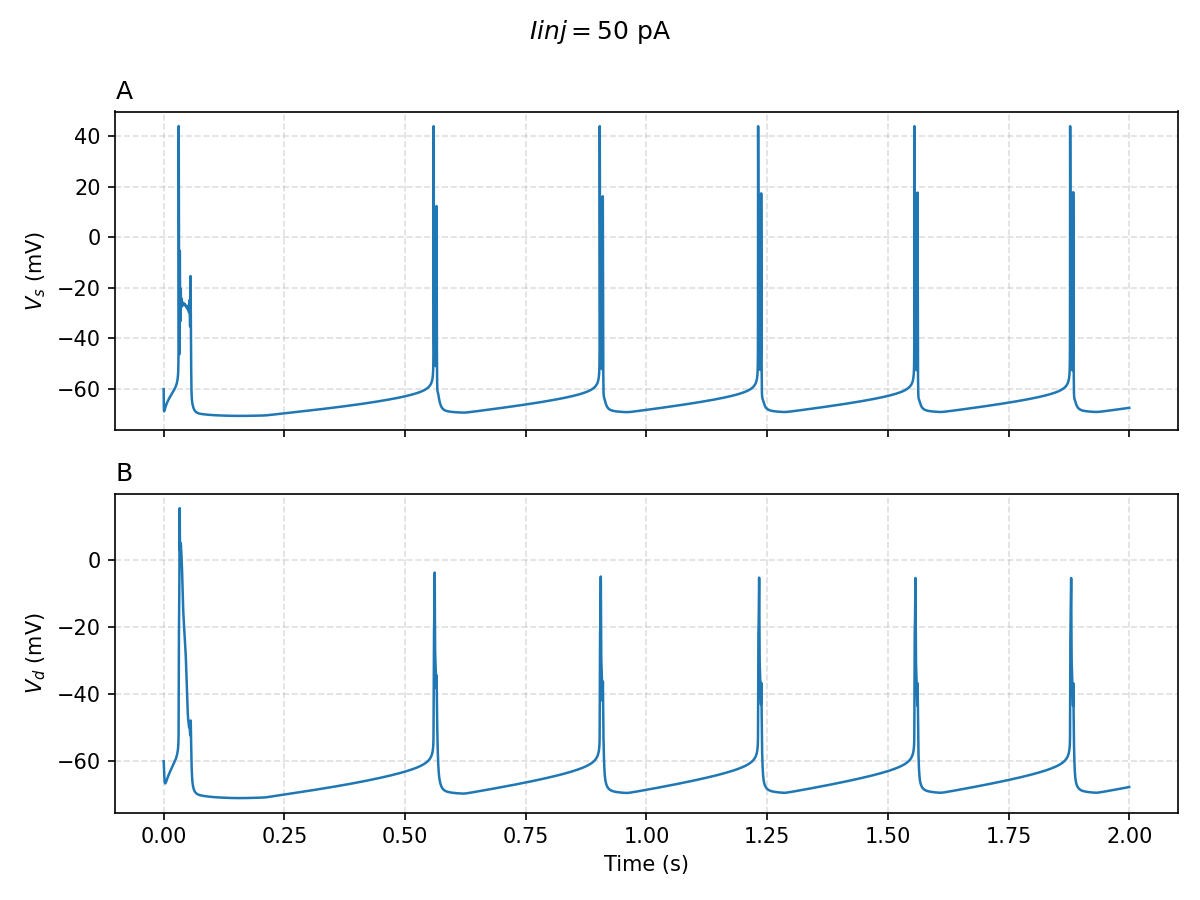
\includegraphics[width=10cm]{../figures/ex_5_I50_dend.png}
		\caption{Gráficos de disparos no soma e no dendrito para corrente $I_{inj} = 50$ nS injetada no dendrito.}
	\end{figure}
	
	\begin{figure}[H]
		\centering
		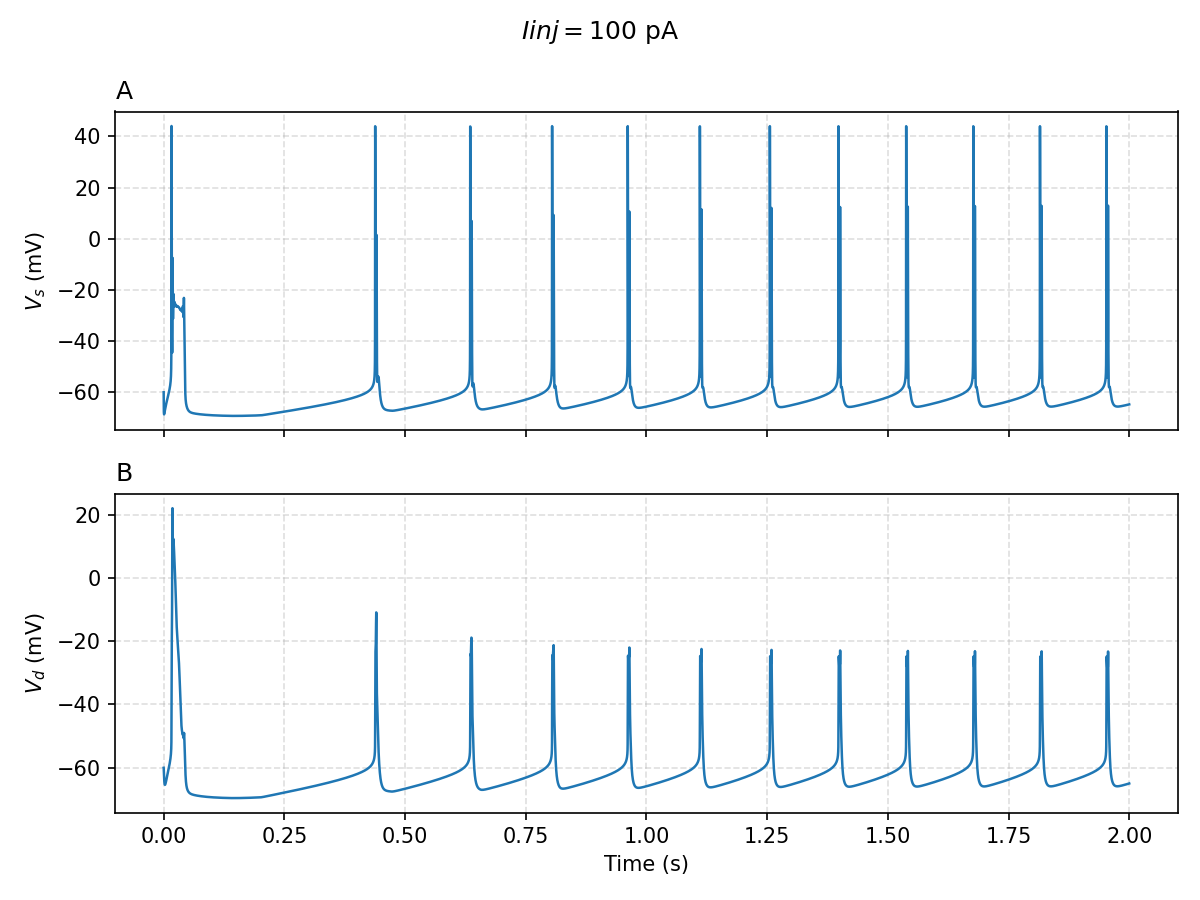
\includegraphics[width=10cm]{../figures/ex_5_I100_dend.png}
		\caption{Gráficos de disparos no soma e no dendrito para corrente $I_{inj} = 100$ nS injetada no dendrito.}
	\end{figure}
	
	\begin{figure}[H]
		\centering
		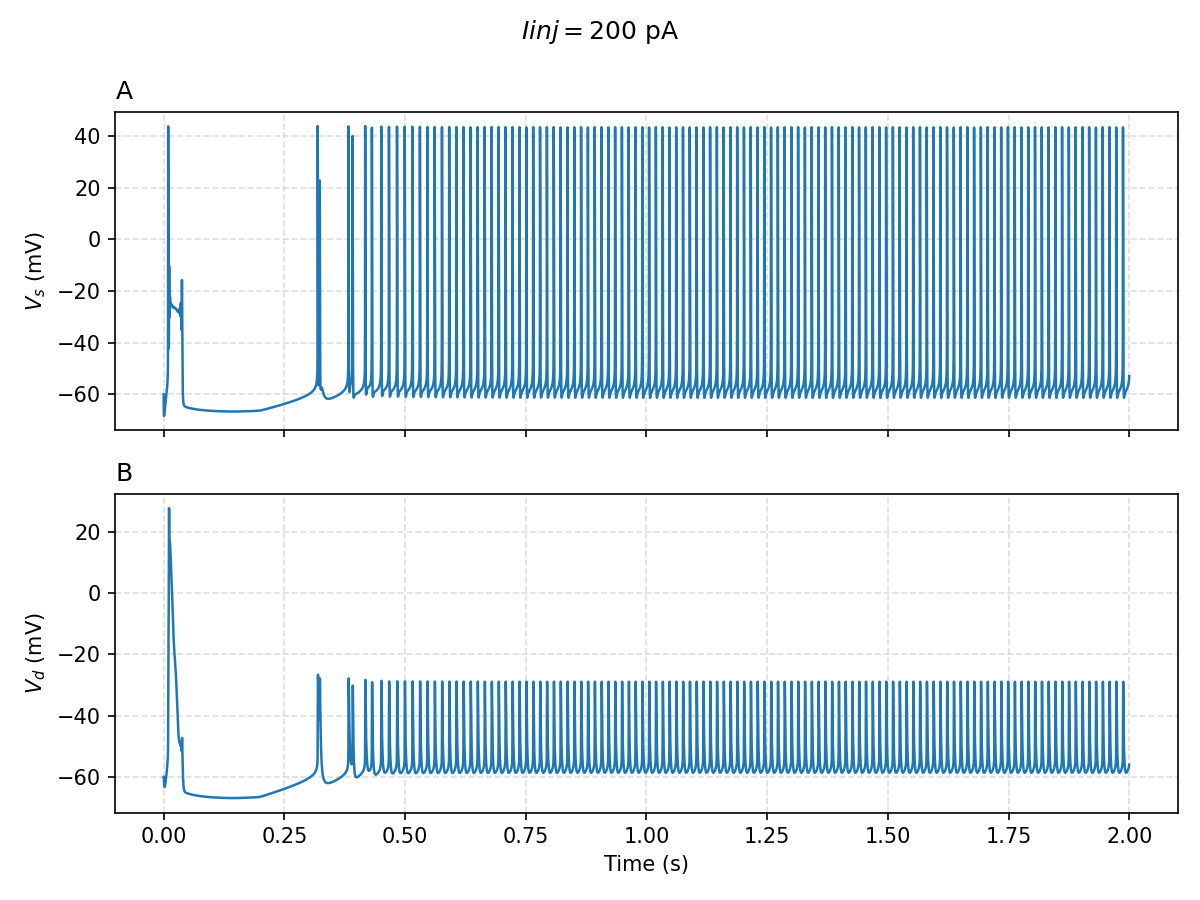
\includegraphics[width=10cm]{../figures/ex_5_I200_dend.png}
		\caption{Gráficos de disparos no soma e no dendrito para corrente $I_{inj} = 200$ nS injetada no dendrito.}
	\end{figure}
	
	A seguir, os gráficos para corrente injetada no soma.
	
	\begin{figure}[H]
		\centering
		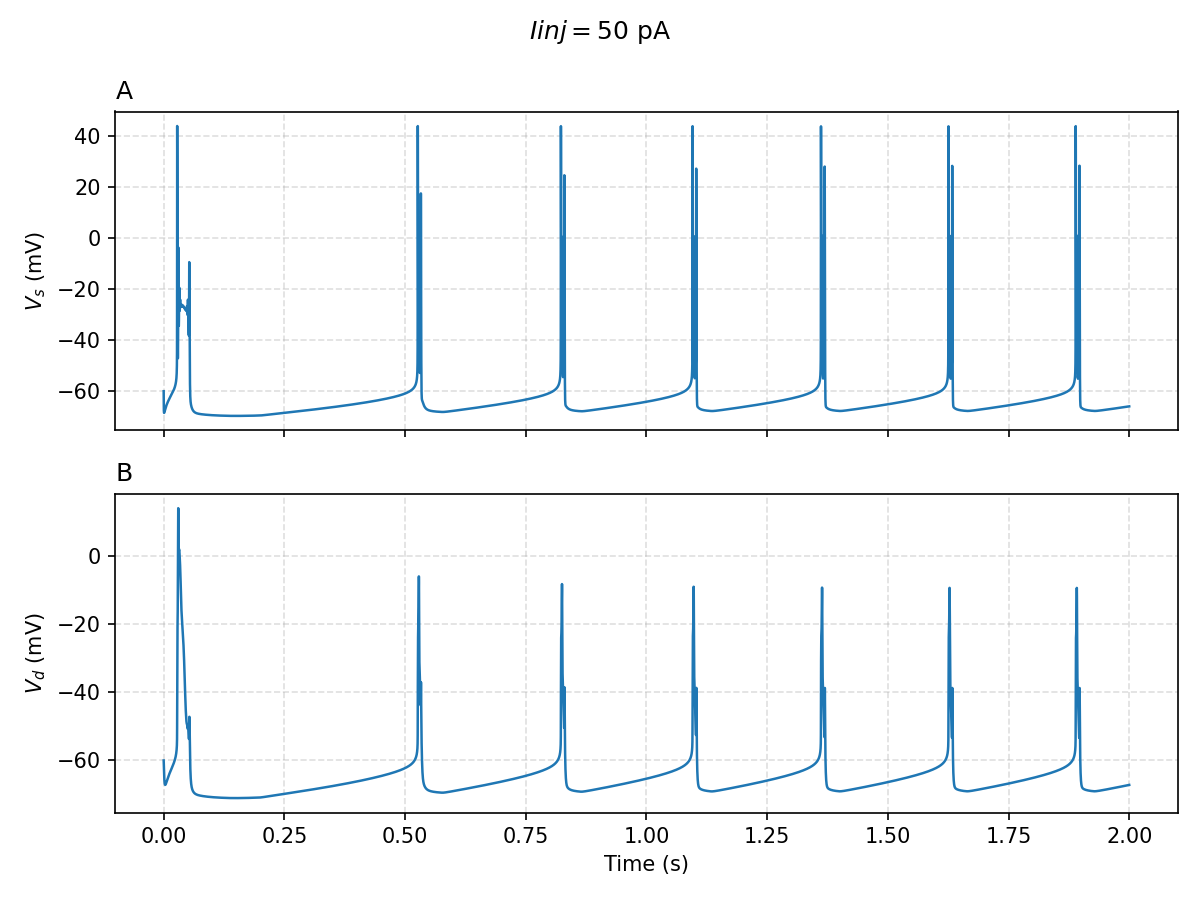
\includegraphics[width=10cm]{../figures/ex_5_I50_soma.png}
		\caption{Gráficos de disparos no soma e no dendrito para corrente $I_{inj} = 50$ nS injetada no soma.}
	\end{figure}
	
	\begin{figure}[H]
		\centering
		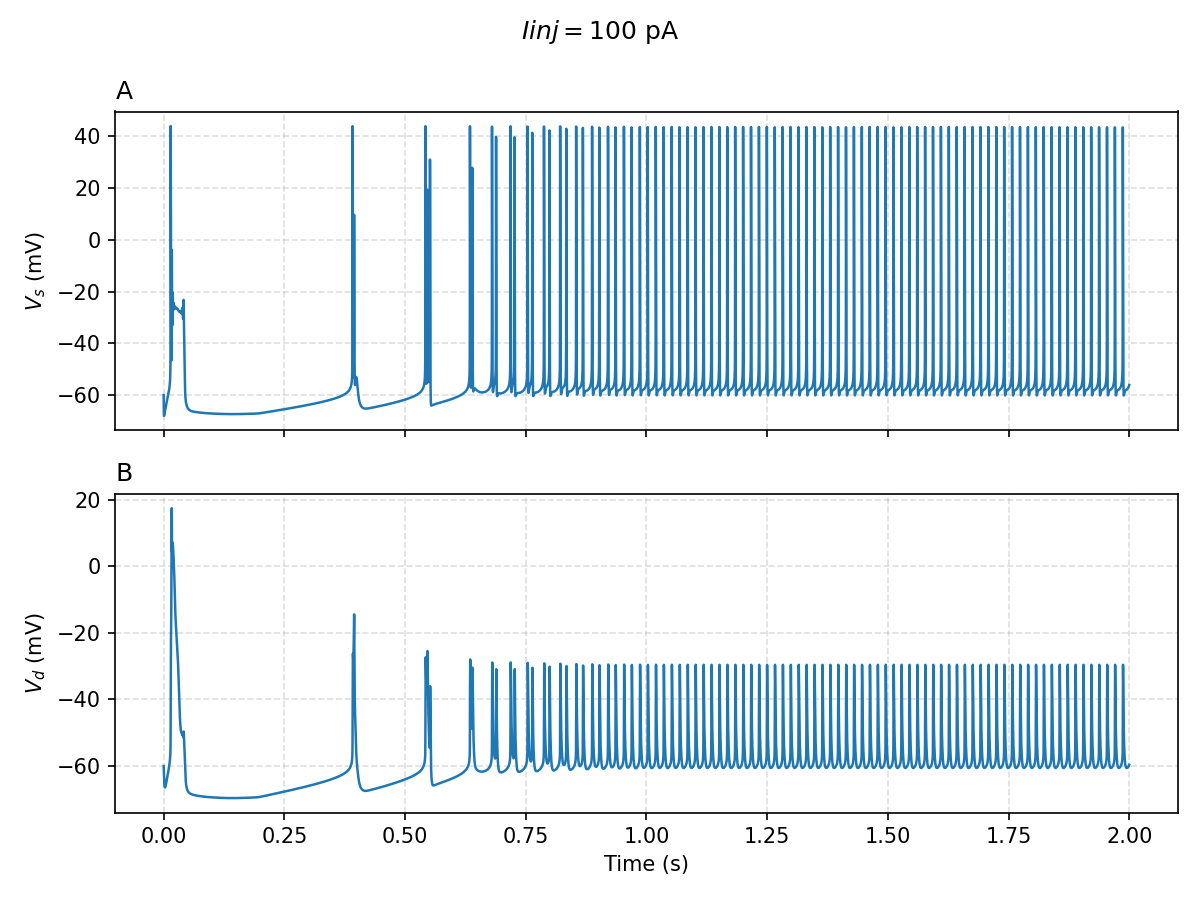
\includegraphics[width=10cm]{../figures/ex_5_I100_soma.png}
		\caption{Gráficos de disparos no soma e no dendrito para corrente $I_{inj} = 100$ nS injetada no soma.}
	\end{figure}
	
	\begin{figure}[H]
		\centering
		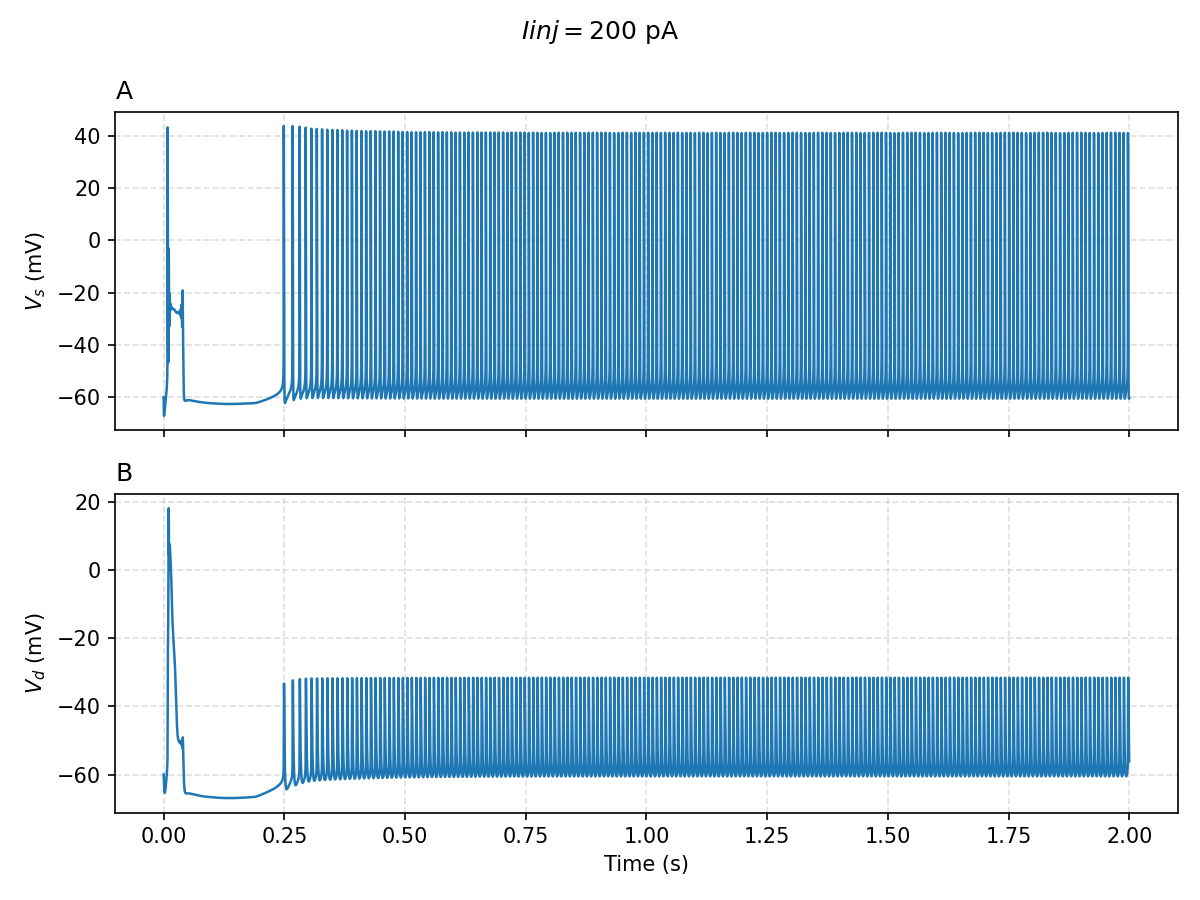
\includegraphics[width=10cm]{../figures/ex_5_I200_soma.png}
		\caption{Gráficos de disparos no soma e no dendrito para corrente $I_{inj} = 200$ nS injetada no soma.}
	\end{figure}
	
	É possível notar que, quando a corrente é injetada diretamente no soma, a frequência de disparos é mais alta, pois quando injetamos no dendrito, a corrente que chega efetivamente no soma para causar os disparos tem menor intensidade e, portanto, menos excitatória.\\\\
	
	\noindent\textbf{Questão 6. (a)} Faça gráficos de $m_{h,\infty}$ e $\tau_{m_h}$ para $-100 \leq V_D \leq 0$.
	
	\begin{figure}[H]
		\centering
		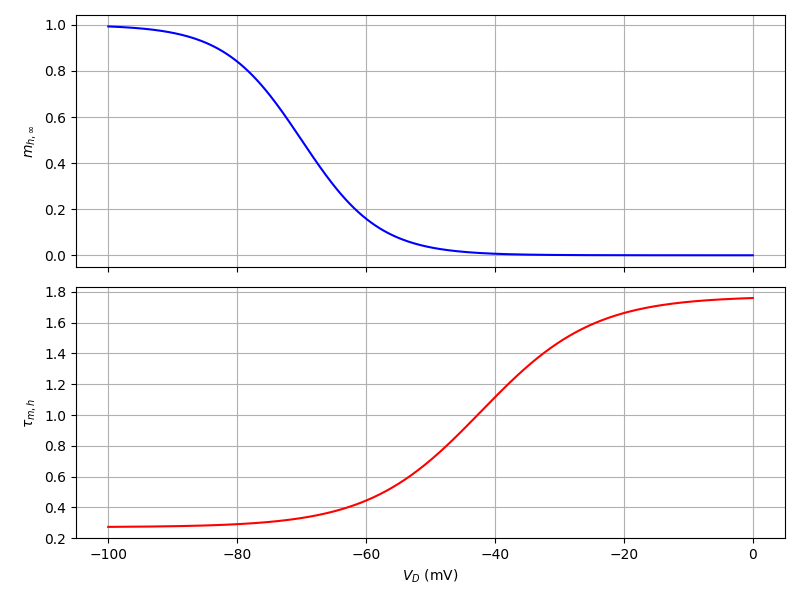
\includegraphics[width=12cm]{../figures/ex_6a.png}
		\caption{Gráficos de $m_{h,\infty}$ e $\tau_{m_h}$ para $-100 \leq V_D \leq 0$.}
	\end{figure}
	
	\noindent\textbf{Questão 6. (b)} Faça um estudo do efeito da condutância $\overline{G}_h$ sobre o intervalo entre rajadas no soma. Use quatro valores diferentes de $\overline{G}_h$: 0, 5 nS, 10 nS e 15 nS. Para cada um desses valores, simule o modelo por 6 segundos e tente gerar gráficos similares aos da Figura 4.18 do livro de Miller (veja uma cópia escaneada dessa figura na Figura 4). Miller mostra gráficos do potencial de membrana somático para $t$ entre 8 e 12 s, mas você pode fazer seus gráficos com $t$ indo de 2 a 6 s. Para produzir gráficos como os da coluna da direita na Figura 4, você terá que definir um critério para o início e o fim de uma rajada. Miller, em seu código em Matlab \texttt{IH\_PR\_loop.m} dado na página web mencionada acima, usa o seguinte critério: uma rajada somática se inicia quando o potencial de membrana dendrítico ultrapassa $V_D = 0$ e termina quando $V_D < -0{,}0500$. Usando este critério (ou algum outro que você defina), determine o instante do início da penúltima rajada de uma simulação $t_{pn}$. Faça agora o gráfico de $V_S$ entre $t_{pn} - 0{,}025$ e $t_{pn} + 0{,}025$ (este será o gráfico em zoom dado na coluna da direita).
	
	\begin{figure}[H]
		\centering
		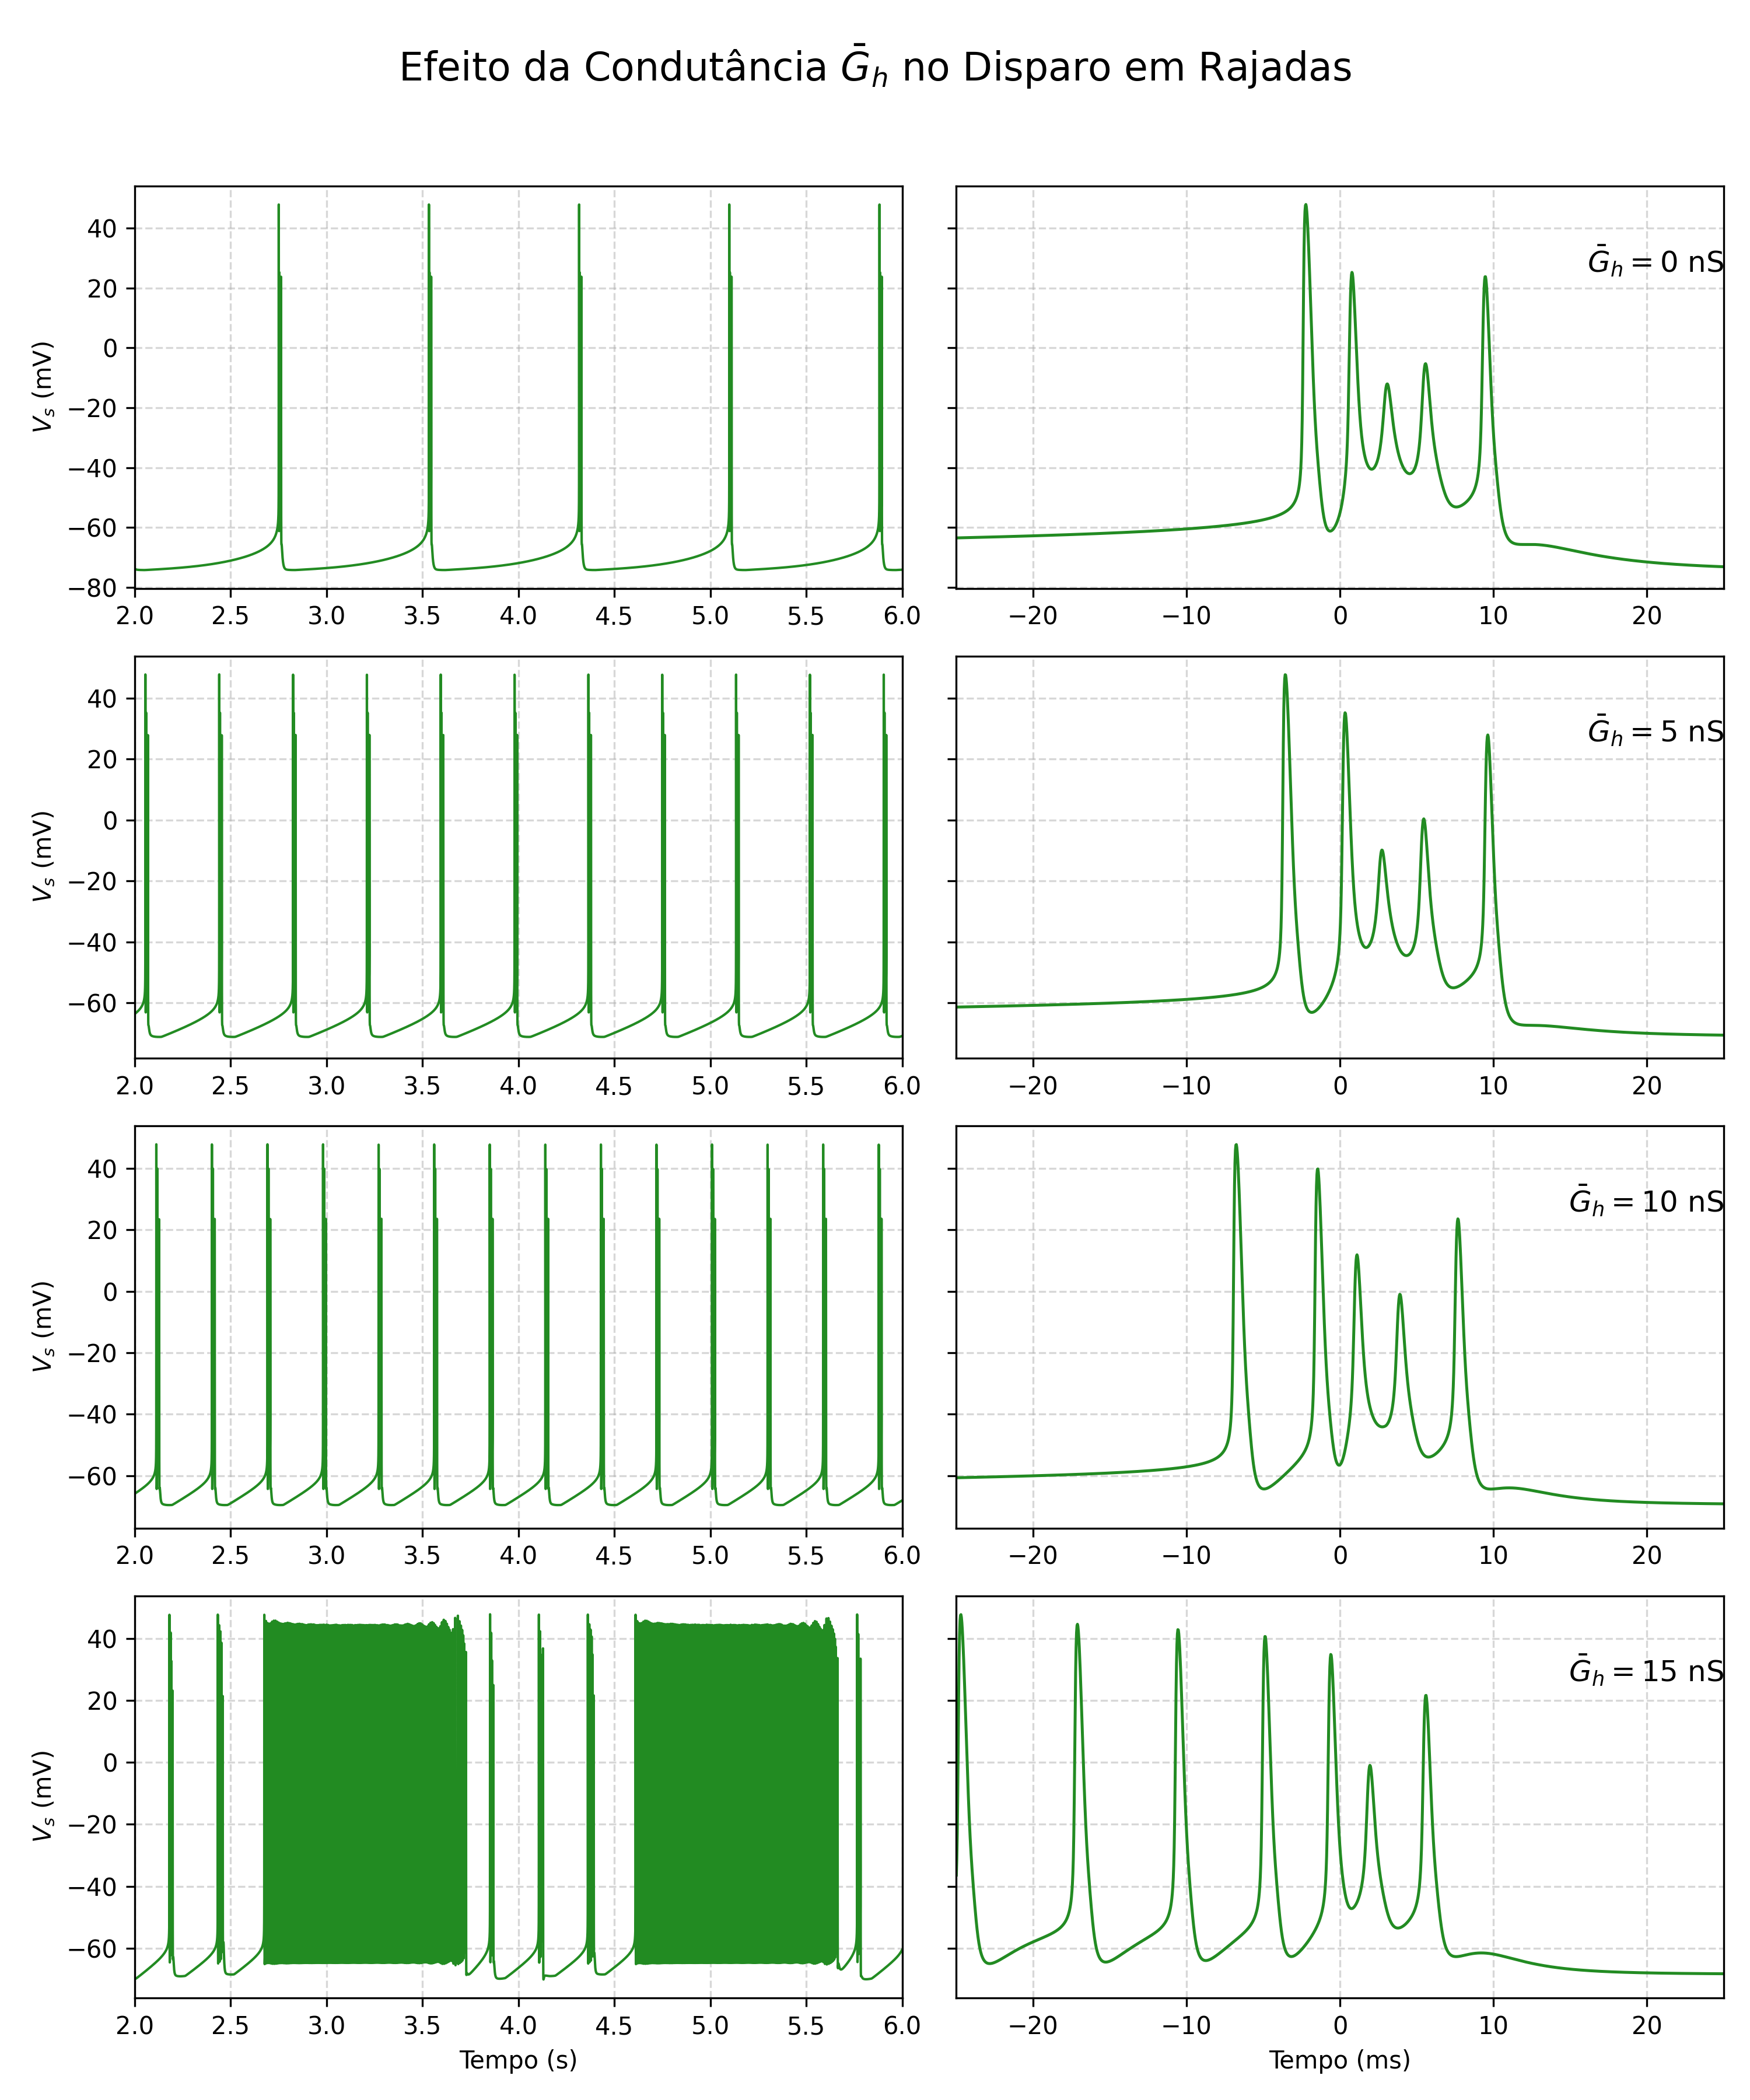
\includegraphics[width=12cm]{../figures/ex_6b.png}
		\caption{Gráficos do estudo da condutância $G_h$..}
	\end{figure}
	
	\noindent\textbf{Questão 6. (c)} Interprete os gráficos gerados por você no item anterior.\\
	
	A condutância de hiperpolarização age aumentando a frequência entre as rajadas e diminuindo a frequência dentro de uma rajada. Além disso, para valores de $G_h$ muito altos, revelam-se regimes tônicos de disparos em determinados momentos. 
	
	
	
	
\end{document}


